
% This LaTeX was auto-generated from MATLAB code.
% To make changes, update the MATLAB code and republish this document.

\documentclass{article}
\usepackage{graphicx}
\usepackage{color}

\sloppy
\definecolor{lightgray}{gray}{0.5}
\setlength{\parindent}{0pt}

\begin{document}

    
    \begin{verbatim}
% plots Julia set for z^2 +c
c= 0.36+.1*1i;   % Define the function whose fixed points we seek.

phiInv= @(z) sqrt(z-c); %this is the inverse iteration of a point

%these holds the real values of the points on the boundary of the filled Julia sets
Rphi=[200^2];
Iphi=[200^2];
arraycount=0;

for j=1:201                  % Try initial values with imaginary parts between
  y = -1+ (j-1)*.01;        %   -1 and 1
  for i=1:201                % and with real parts between
    x = -1 + (i-1)*.01;     %   -1 and 1.
    arraycount=arraycount+1; %increment the Iphi/Rphi arraycount
    zk=x+y*1i;      %set zk to the point in the [-1,1]x[-1,1] region
    kcount=0;       %counter for reverse iteration

    %run reverse iteration untill it reaches boundary, kick out if it
    %diverges
    while kcount < 100 && abs(zk) < 2
      n=randi(2,1);
      y=imag(zk-c);
      kcount = kcount+1;
      zk=(-1)^n*phiInv(zk);

    end
    %zk is now on the boundary, so set the real and imaginary arrays to its
    %value there
    if abs(zk)<2
    Rphi(arraycount)=real(zk);
    Iphi(arraycount)=imag(zk);
    end
  end
end
%plot the Rphi vs Iphi
scatter(Rphi,Iphi,'.')
pbaspect([1 1 1]);  %keep aspect ration square

%{

image([-1.8 1.8],[-1.8 1.8],M),  % This plots the results.
pbaspect([1 1 1]); %keeps the x/y ratio even
axis xy            % If you don't do this, vertical axis is inverted.

%}
\end{verbatim}

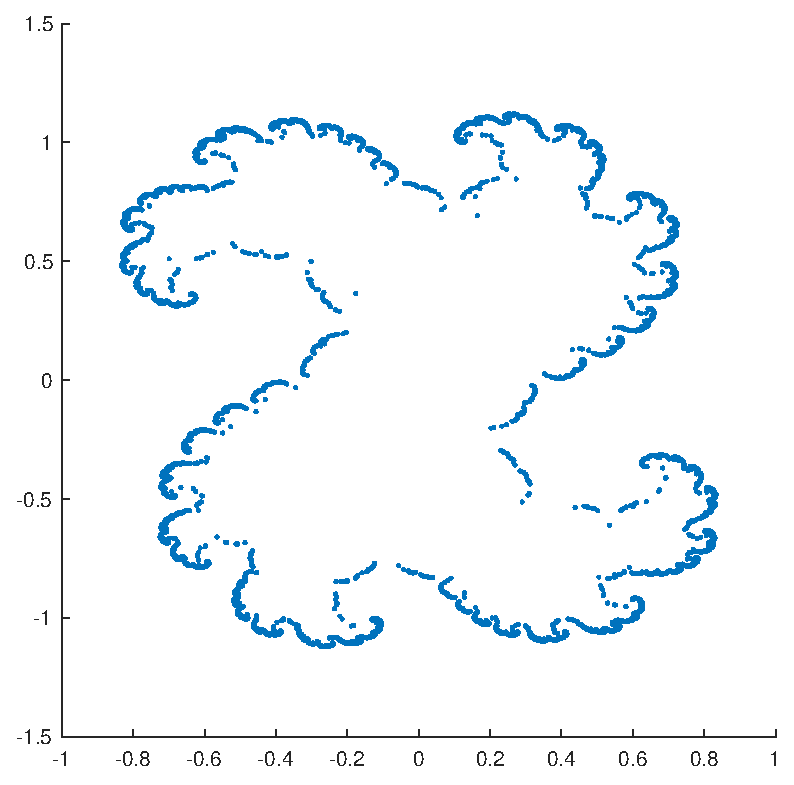
\includegraphics [width=4in]{JuliaBound3_01.eps}



\end{document}
    
